\documentclass[10pt]{article}
% Anonymous / double-blind TMLR submission (no accepted/preprint option).
\usepackage{tmlr}
%%%%% NEW MATH DEFINITIONS %%%%%

\usepackage{amsmath,amsfonts,bm}

% Mark sections of captions for referring to divisions of figures
\newcommand{\figleft}{{\em (Left)}}
\newcommand{\figcenter}{{\em (Center)}}
\newcommand{\figright}{{\em (Right)}}
\newcommand{\figtop}{{\em (Top)}}
\newcommand{\figbottom}{{\em (Bottom)}}
\newcommand{\captiona}{{\em (a)}}
\newcommand{\captionb}{{\em (b)}}
\newcommand{\captionc}{{\em (c)}}
\newcommand{\captiond}{{\em (d)}}

% Highlight a newly defined term
\newcommand{\newterm}[1]{{\bf #1}}


% Figure reference, lower-case.
\def\figref#1{figure~\ref{#1}}
% Figure reference, capital. For start of sentence
\def\Figref#1{Figure~\ref{#1}}
\def\twofigref#1#2{figures \ref{#1} and \ref{#2}}
\def\quadfigref#1#2#3#4{figures \ref{#1}, \ref{#2}, \ref{#3} and \ref{#4}}
% Section reference, lower-case.
\def\secref#1{section~\ref{#1}}
% Section reference, capital.
\def\Secref#1{Section~\ref{#1}}
% Reference to two sections.
\def\twosecrefs#1#2{sections \ref{#1} and \ref{#2}}
% Reference to three sections.
\def\secrefs#1#2#3{sections \ref{#1}, \ref{#2} and \ref{#3}}
% Reference to an equation, lower-case.
\def\eqref#1{equation~\ref{#1}}
% Reference to an equation, upper case
\def\Eqref#1{Equation~\ref{#1}}
% A raw reference to an equation---avoid using if possible
\def\plaineqref#1{\ref{#1}}
% Reference to a chapter, lower-case.
\def\chapref#1{chapter~\ref{#1}}
% Reference to an equation, upper case.
\def\Chapref#1{Chapter~\ref{#1}}
% Reference to a range of chapters
\def\rangechapref#1#2{chapters\ref{#1}--\ref{#2}}
% Reference to an algorithm, lower-case.
\def\algref#1{algorithm~\ref{#1}}
% Reference to an algorithm, upper case.
\def\Algref#1{Algorithm~\ref{#1}}
\def\twoalgref#1#2{algorithms \ref{#1} and \ref{#2}}
\def\Twoalgref#1#2{Algorithms \ref{#1} and \ref{#2}}
% Reference to a part, lower case
\def\partref#1{part~\ref{#1}}
% Reference to a part, upper case
\def\Partref#1{Part~\ref{#1}}
\def\twopartref#1#2{parts \ref{#1} and \ref{#2}}

\def\ceil#1{\lceil #1 \rceil}
\def\floor#1{\lfloor #1 \rfloor}
\def\1{\bm{1}}
\newcommand{\train}{\mathcal{D}}
\newcommand{\valid}{\mathcal{D_{\mathrm{valid}}}}
\newcommand{\test}{\mathcal{D_{\mathrm{test}}}}

\def\eps{{\epsilon}}


% Random variables
\def\reta{{\textnormal{$\eta$}}}
\def\ra{{\textnormal{a}}}
\def\rb{{\textnormal{b}}}
\def\rc{{\textnormal{c}}}
\def\rd{{\textnormal{d}}}
\def\re{{\textnormal{e}}}
\def\rf{{\textnormal{f}}}
\def\rg{{\textnormal{g}}}
\def\rh{{\textnormal{h}}}
\def\ri{{\textnormal{i}}}
\def\rj{{\textnormal{j}}}
\def\rk{{\textnormal{k}}}
\def\rl{{\textnormal{l}}}
% rm is already a command, just don't name any random variables m
\def\rn{{\textnormal{n}}}
\def\ro{{\textnormal{o}}}
\def\rp{{\textnormal{p}}}
\def\rq{{\textnormal{q}}}
\def\rr{{\textnormal{r}}}
\def\rs{{\textnormal{s}}}
\def\rt{{\textnormal{t}}}
\def\ru{{\textnormal{u}}}
\def\rv{{\textnormal{v}}}
\def\rw{{\textnormal{w}}}
\def\rx{{\textnormal{x}}}
\def\ry{{\textnormal{y}}}
\def\rz{{\textnormal{z}}}

% Random vectors
\def\rvepsilon{{\mathbf{\epsilon}}}
\def\rvtheta{{\mathbf{\theta}}}
\def\rva{{\mathbf{a}}}
\def\rvb{{\mathbf{b}}}
\def\rvc{{\mathbf{c}}}
\def\rvd{{\mathbf{d}}}
\def\rve{{\mathbf{e}}}
\def\rvf{{\mathbf{f}}}
\def\rvg{{\mathbf{g}}}
\def\rvh{{\mathbf{h}}}
\def\rvu{{\mathbf{i}}}
\def\rvj{{\mathbf{j}}}
\def\rvk{{\mathbf{k}}}
\def\rvl{{\mathbf{l}}}
\def\rvm{{\mathbf{m}}}
\def\rvn{{\mathbf{n}}}
\def\rvo{{\mathbf{o}}}
\def\rvp{{\mathbf{p}}}
\def\rvq{{\mathbf{q}}}
\def\rvr{{\mathbf{r}}}
\def\rvs{{\mathbf{s}}}
\def\rvt{{\mathbf{t}}}
\def\rvu{{\mathbf{u}}}
\def\rvv{{\mathbf{v}}}
\def\rvw{{\mathbf{w}}}
\def\rvx{{\mathbf{x}}}
\def\rvy{{\mathbf{y}}}
\def\rvz{{\mathbf{z}}}

% Elements of random vectors
\def\erva{{\textnormal{a}}}
\def\ervb{{\textnormal{b}}}
\def\ervc{{\textnormal{c}}}
\def\ervd{{\textnormal{d}}}
\def\erve{{\textnormal{e}}}
\def\ervf{{\textnormal{f}}}
\def\ervg{{\textnormal{g}}}
\def\ervh{{\textnormal{h}}}
\def\ervi{{\textnormal{i}}}
\def\ervj{{\textnormal{j}}}
\def\ervk{{\textnormal{k}}}
\def\ervl{{\textnormal{l}}}
\def\ervm{{\textnormal{m}}}
\def\ervn{{\textnormal{n}}}
\def\ervo{{\textnormal{o}}}
\def\ervp{{\textnormal{p}}}
\def\ervq{{\textnormal{q}}}
\def\ervr{{\textnormal{r}}}
\def\ervs{{\textnormal{s}}}
\def\ervt{{\textnormal{t}}}
\def\ervu{{\textnormal{u}}}
\def\ervv{{\textnormal{v}}}
\def\ervw{{\textnormal{w}}}
\def\ervx{{\textnormal{x}}}
\def\ervy{{\textnormal{y}}}
\def\ervz{{\textnormal{z}}}

% Random matrices
\def\rmA{{\mathbf{A}}}
\def\rmB{{\mathbf{B}}}
\def\rmC{{\mathbf{C}}}
\def\rmD{{\mathbf{D}}}
\def\rmE{{\mathbf{E}}}
\def\rmF{{\mathbf{F}}}
\def\rmG{{\mathbf{G}}}
\def\rmH{{\mathbf{H}}}
\def\rmI{{\mathbf{I}}}
\def\rmJ{{\mathbf{J}}}
\def\rmK{{\mathbf{K}}}
\def\rmL{{\mathbf{L}}}
\def\rmM{{\mathbf{M}}}
\def\rmN{{\mathbf{N}}}
\def\rmO{{\mathbf{O}}}
\def\rmP{{\mathbf{P}}}
\def\rmQ{{\mathbf{Q}}}
\def\rmR{{\mathbf{R}}}
\def\rmS{{\mathbf{S}}}
\def\rmT{{\mathbf{T}}}
\def\rmU{{\mathbf{U}}}
\def\rmV{{\mathbf{V}}}
\def\rmW{{\mathbf{W}}}
\def\rmX{{\mathbf{X}}}
\def\rmY{{\mathbf{Y}}}
\def\rmZ{{\mathbf{Z}}}

% Elements of random matrices
\def\ermA{{\textnormal{A}}}
\def\ermB{{\textnormal{B}}}
\def\ermC{{\textnormal{C}}}
\def\ermD{{\textnormal{D}}}
\def\ermE{{\textnormal{E}}}
\def\ermF{{\textnormal{F}}}
\def\ermG{{\textnormal{G}}}
\def\ermH{{\textnormal{H}}}
\def\ermI{{\textnormal{I}}}
\def\ermJ{{\textnormal{J}}}
\def\ermK{{\textnormal{K}}}
\def\ermL{{\textnormal{L}}}
\def\ermM{{\textnormal{M}}}
\def\ermN{{\textnormal{N}}}
\def\ermO{{\textnormal{O}}}
\def\ermP{{\textnormal{P}}}
\def\ermQ{{\textnormal{Q}}}
\def\ermR{{\textnormal{R}}}
\def\ermS{{\textnormal{S}}}
\def\ermT{{\textnormal{T}}}
\def\ermU{{\textnormal{U}}}
\def\ermV{{\textnormal{V}}}
\def\ermW{{\textnormal{W}}}
\def\ermX{{\textnormal{X}}}
\def\ermY{{\textnormal{Y}}}
\def\ermZ{{\textnormal{Z}}}

% Vectors
\def\vzero{{\bm{0}}}
\def\vone{{\bm{1}}}
\def\vmu{{\bm{\mu}}}
\def\vtheta{{\bm{\theta}}}
\def\va{{\bm{a}}}
\def\vb{{\bm{b}}}
\def\vc{{\bm{c}}}
\def\vd{{\bm{d}}}
\def\ve{{\bm{e}}}
\def\vf{{\bm{f}}}
\def\vg{{\bm{g}}}
\def\vh{{\bm{h}}}
\def\vi{{\bm{i}}}
\def\vj{{\bm{j}}}
\def\vk{{\bm{k}}}
\def\vl{{\bm{l}}}
\def\vm{{\bm{m}}}
\def\vn{{\bm{n}}}
\def\vo{{\bm{o}}}
\def\vp{{\bm{p}}}
\def\vq{{\bm{q}}}
\def\vr{{\bm{r}}}
\def\vs{{\bm{s}}}
\def\vt{{\bm{t}}}
\def\vu{{\bm{u}}}
\def\vv{{\bm{v}}}
\def\vw{{\bm{w}}}
\def\vx{{\bm{x}}}
\def\vy{{\bm{y}}}
\def\vz{{\bm{z}}}

% Elements of vectors
\def\evalpha{{\alpha}}
\def\evbeta{{\beta}}
\def\evepsilon{{\epsilon}}
\def\evlambda{{\lambda}}
\def\evomega{{\omega}}
\def\evmu{{\mu}}
\def\evpsi{{\psi}}
\def\evsigma{{\sigma}}
\def\evtheta{{\theta}}
\def\eva{{a}}
\def\evb{{b}}
\def\evc{{c}}
\def\evd{{d}}
\def\eve{{e}}
\def\evf{{f}}
\def\evg{{g}}
\def\evh{{h}}
\def\evi{{i}}
\def\evj{{j}}
\def\evk{{k}}
\def\evl{{l}}
\def\evm{{m}}
\def\evn{{n}}
\def\evo{{o}}
\def\evp{{p}}
\def\evq{{q}}
\def\evr{{r}}
\def\evs{{s}}
\def\evt{{t}}
\def\evu{{u}}
\def\evv{{v}}
\def\evw{{w}}
\def\evx{{x}}
\def\evy{{y}}
\def\evz{{z}}

% Matrix
\def\mA{{\bm{A}}}
\def\mB{{\bm{B}}}
\def\mC{{\bm{C}}}
\def\mD{{\bm{D}}}
\def\mE{{\bm{E}}}
\def\mF{{\bm{F}}}
\def\mG{{\bm{G}}}
\def\mH{{\bm{H}}}
\def\mI{{\bm{I}}}
\def\mJ{{\bm{J}}}
\def\mK{{\bm{K}}}
\def\mL{{\bm{L}}}
\def\mM{{\bm{M}}}
\def\mN{{\bm{N}}}
\def\mO{{\bm{O}}}
\def\mP{{\bm{P}}}
\def\mQ{{\bm{Q}}}
\def\mR{{\bm{R}}}
\def\mS{{\bm{S}}}
\def\mT{{\bm{T}}}
\def\mU{{\bm{U}}}
\def\mV{{\bm{V}}}
\def\mW{{\bm{W}}}
\def\mX{{\bm{X}}}
\def\mY{{\bm{Y}}}
\def\mZ{{\bm{Z}}}
\def\mBeta{{\bm{\beta}}}
\def\mPhi{{\bm{\Phi}}}
\def\mLambda{{\bm{\Lambda}}}
\def\mSigma{{\bm{\Sigma}}}

% Tensor
\DeclareMathAlphabet{\mathsfit}{\encodingdefault}{\sfdefault}{m}{sl}
\SetMathAlphabet{\mathsfit}{bold}{\encodingdefault}{\sfdefault}{bx}{n}
\newcommand{\tens}[1]{\bm{\mathsfit{#1}}}
\def\tA{{\tens{A}}}
\def\tB{{\tens{B}}}
\def\tC{{\tens{C}}}
\def\tD{{\tens{D}}}
\def\tE{{\tens{E}}}
\def\tF{{\tens{F}}}
\def\tG{{\tens{G}}}
\def\tH{{\tens{H}}}
\def\tI{{\tens{I}}}
\def\tJ{{\tens{J}}}
\def\tK{{\tens{K}}}
\def\tL{{\tens{L}}}
\def\tM{{\tens{M}}}
\def\tN{{\tens{N}}}
\def\tO{{\tens{O}}}
\def\tP{{\tens{P}}}
\def\tQ{{\tens{Q}}}
\def\tR{{\tens{R}}}
\def\tS{{\tens{S}}}
\def\tT{{\tens{T}}}
\def\tU{{\tens{U}}}
\def\tV{{\tens{V}}}
\def\tW{{\tens{W}}}
\def\tX{{\tens{X}}}
\def\tY{{\tens{Y}}}
\def\tZ{{\tens{Z}}}


% Graph
\def\gA{{\mathcal{A}}}
\def\gB{{\mathcal{B}}}
\def\gC{{\mathcal{C}}}
\def\gD{{\mathcal{D}}}
\def\gE{{\mathcal{E}}}
\def\gF{{\mathcal{F}}}
\def\gG{{\mathcal{G}}}
\def\gH{{\mathcal{H}}}
\def\gI{{\mathcal{I}}}
\def\gJ{{\mathcal{J}}}
\def\gK{{\mathcal{K}}}
\def\gL{{\mathcal{L}}}
\def\gM{{\mathcal{M}}}
\def\gN{{\mathcal{N}}}
\def\gO{{\mathcal{O}}}
\def\gP{{\mathcal{P}}}
\def\gQ{{\mathcal{Q}}}
\def\gR{{\mathcal{R}}}
\def\gS{{\mathcal{S}}}
\def\gT{{\mathcal{T}}}
\def\gU{{\mathcal{U}}}
\def\gV{{\mathcal{V}}}
\def\gW{{\mathcal{W}}}
\def\gX{{\mathcal{X}}}
\def\gY{{\mathcal{Y}}}
\def\gZ{{\mathcal{Z}}}

% Sets
\def\sA{{\mathbb{A}}}
\def\sB{{\mathbb{B}}}
\def\sC{{\mathbb{C}}}
\def\sD{{\mathbb{D}}}
% Don't use a set called E, because this would be the same as our symbol
% for expectation.
\def\sF{{\mathbb{F}}}
\def\sG{{\mathbb{G}}}
\def\sH{{\mathbb{H}}}
\def\sI{{\mathbb{I}}}
\def\sJ{{\mathbb{J}}}
\def\sK{{\mathbb{K}}}
\def\sL{{\mathbb{L}}}
\def\sM{{\mathbb{M}}}
\def\sN{{\mathbb{N}}}
\def\sO{{\mathbb{O}}}
\def\sP{{\mathbb{P}}}
\def\sQ{{\mathbb{Q}}}
\def\sR{{\mathbb{R}}}
\def\sS{{\mathbb{S}}}
\def\sT{{\mathbb{T}}}
\def\sU{{\mathbb{U}}}
\def\sV{{\mathbb{V}}}
\def\sW{{\mathbb{W}}}
\def\sX{{\mathbb{X}}}
\def\sY{{\mathbb{Y}}}
\def\sZ{{\mathbb{Z}}}

% Entries of a matrix
\def\emLambda{{\Lambda}}
\def\emA{{A}}
\def\emB{{B}}
\def\emC{{C}}
\def\emD{{D}}
\def\emE{{E}}
\def\emF{{F}}
\def\emG{{G}}
\def\emH{{H}}
\def\emI{{I}}
\def\emJ{{J}}
\def\emK{{K}}
\def\emL{{L}}
\def\emM{{M}}
\def\emN{{N}}
\def\emO{{O}}
\def\emP{{P}}
\def\emQ{{Q}}
\def\emR{{R}}
\def\emS{{S}}
\def\emT{{T}}
\def\emU{{U}}
\def\emV{{V}}
\def\emW{{W}}
\def\emX{{X}}
\def\emY{{Y}}
\def\emZ{{Z}}
\def\emSigma{{\Sigma}}

% entries of a tensor
% Same font as tensor, without \bm wrapper
\newcommand{\etens}[1]{\mathsfit{#1}}
\def\etLambda{{\etens{\Lambda}}}
\def\etA{{\etens{A}}}
\def\etB{{\etens{B}}}
\def\etC{{\etens{C}}}
\def\etD{{\etens{D}}}
\def\etE{{\etens{E}}}
\def\etF{{\etens{F}}}
\def\etG{{\etens{G}}}
\def\etH{{\etens{H}}}
\def\etI{{\etens{I}}}
\def\etJ{{\etens{J}}}
\def\etK{{\etens{K}}}
\def\etL{{\etens{L}}}
\def\etM{{\etens{M}}}
\def\etN{{\etens{N}}}
\def\etO{{\etens{O}}}
\def\etP{{\etens{P}}}
\def\etQ{{\etens{Q}}}
\def\etR{{\etens{R}}}
\def\etS{{\etens{S}}}
\def\etT{{\etens{T}}}
\def\etU{{\etens{U}}}
\def\etV{{\etens{V}}}
\def\etW{{\etens{W}}}
\def\etX{{\etens{X}}}
\def\etY{{\etens{Y}}}
\def\etZ{{\etens{Z}}}

% The true underlying data generating distribution
\newcommand{\pdata}{p_{\rm{data}}}
% The empirical distribution defined by the training set
\newcommand{\ptrain}{\hat{p}_{\rm{data}}}
\newcommand{\Ptrain}{\hat{P}_{\rm{data}}}
% The model distribution
\newcommand{\pmodel}{p_{\rm{model}}}
\newcommand{\Pmodel}{P_{\rm{model}}}
\newcommand{\ptildemodel}{\tilde{p}_{\rm{model}}}
% Stochastic autoencoder distributions
\newcommand{\pencode}{p_{\rm{encoder}}}
\newcommand{\pdecode}{p_{\rm{decoder}}}
\newcommand{\precons}{p_{\rm{reconstruct}}}

\newcommand{\laplace}{\mathrm{Laplace}} % Laplace distribution

\newcommand{\E}{\mathbb{E}}
\newcommand{\Ls}{\mathcal{L}}
\newcommand{\R}{\mathbb{R}}
\newcommand{\emp}{\tilde{p}}
\newcommand{\lr}{\alpha}
\newcommand{\reg}{\lambda}
\newcommand{\rect}{\mathrm{rectifier}}
\newcommand{\softmax}{\mathrm{softmax}}
\newcommand{\sigmoid}{\sigma}
\newcommand{\softplus}{\zeta}
\newcommand{\KL}{D_{\mathrm{KL}}}
\newcommand{\Var}{\mathrm{Var}}
\newcommand{\standarderror}{\mathrm{SE}}
\newcommand{\Cov}{\mathrm{Cov}}
% Wolfram Mathworld says $L^2$ is for function spaces and $\ell^2$ is for vectors
% But then they seem to use $L^2$ for vectors throughout the site, and so does
% wikipedia.
\newcommand{\normlzero}{L^0}
\newcommand{\normlone}{L^1}
\newcommand{\normltwo}{L^2}
\newcommand{\normlp}{L^p}
\newcommand{\normmax}{L^\infty}

\newcommand{\parents}{Pa} % See usage in notation.tex. Chosen to match Daphne's book.

\DeclareMathOperator*{\argmax}{arg\,max}
\DeclareMathOperator*{\argmin}{arg\,min}

\DeclareMathOperator{\sign}{sign}
\DeclareMathOperator{\Tr}{Tr}
\let\ab\allowbreak


\usepackage{hyperref}
\usepackage{url}
\usepackage{booktabs}
\usepackage{graphicx}
\usepackage{xspace}
\usepackage{xcolor}

% Blank PDF identity metadata (anonymization).
\hypersetup{
  pdfauthor={},
  pdfcreator={},
  pdfproducer={},
  pdfsubject={},
  pdfkeywords={}
}

% Auto-generated by scripts/make_numbers.py — do not edit by hand.
% Every macro is sourced from an existing result JSON (see numbers_sources.csv).

\newcommand{\CoreMZero}{0.691}
\newcommand{\CoreMZeroCI}{[0.652, 0.731]}
\newcommand{\CoreMOne}{0.752}
\newcommand{\CoreMOneCI}{[0.691, 0.806]}
\newcommand{\CoreMTwo}{0.798}
\newcommand{\CoreMTwoCI}{[0.746, 0.842]}
\newcommand{\CoreDelta}{0.107}
\newcommand{\CoreDeltaCI}{[0.073, 0.143]}
\newcommand{\CoreMOneKOne}{0.794}
\newcommand{\CoreMOneKTwo}{0.687}
\newcommand{\CoreMOneKThree}{0.777}
\newcommand{\CoreWithinPersonMOne}{0.761}
\newcommand{\CoreWithinPersonMOneCI}{[0.694, 0.819]}
\newcommand{\CoreBaseEpochZeroMOne}{0.468}
\newcommand{\CoreBaseEpochZeroMOneCI}{[0.429, 0.508]}
\newcommand{\CorePeakLayer}{13}
\newcommand{\CorePeakMOne}{0.767}
\newcommand{\CorePeakMOneCI}{[0.700, 0.821]}
\newcommand{\StrengthNKOne}{72}
\newcommand{\StrengthMZeroKOne}{0.539}
\newcommand{\StrengthMOneKOne}{0.755}
\newcommand{\RegionKOne}{0.778}
\newcommand{\RegionKOneCI}{[0.727, 0.831]}
\newcommand{\ValueBirKOne}{0.647}
\newcommand{\ValueEmpKOne}{0.555}
\newcommand{\ValueUniKOne}{0.625}
\newcommand{\ValueHobKOne}{0.665}
\newcommand{\StrengthNKTwo}{52}
\newcommand{\StrengthMZeroKTwo}{0.556}
\newcommand{\StrengthMOneKTwo}{0.747}
\newcommand{\RegionKTwo}{0.694}
\newcommand{\RegionKTwoCI}{[0.633, 0.758]}
\newcommand{\ValueBirKTwo}{0.615}
\newcommand{\ValueEmpKTwo}{0.565}
\newcommand{\ValueUniKTwo}{0.585}
\newcommand{\ValueHobKTwo}{0.592}
\newcommand{\StrengthNKThree}{126}
\newcommand{\StrengthMZeroKThree}{0.522}
\newcommand{\StrengthMOneKThree}{0.772}
\newcommand{\RegionKThree}{0.882}
\newcommand{\RegionKThreeCI}{[0.844, 0.917]}
\newcommand{\ValueBirKThree}{0.670}
\newcommand{\ValueEmpKThree}{0.580}
\newcommand{\ValueUniKThree}{0.592}
\newcommand{\ValueHobKThree}{0.628}
\newcommand{\StackedDeltaKOne}{0.046}
\newcommand{\StackedDeltaKTwo}{0.055}
\newcommand{\StackedDeltaKThree}{0.075}
\newcommand{\ProbeJOneMin}{0.437}
\newcommand{\ProbeJOneMax}{0.513}
\newcommand{\ProbeJFourMin}{0.448}
\newcommand{\ProbeJFourMax}{0.528}
\newcommand{\AnchorIdAurocMin}{1.000}
\newcommand{\AnchorIdAurocMax}{1.000}
\newcommand{\LeakAurocMin}{0.476}
\newcommand{\LeakAurocMax}{0.511}
\newcommand{\CoreArmMOne}{0.752}
\newcommand{\CoreArmMOneCI}{[0.691, 0.806]}
\newcommand{\CoreMOneDEBUNKDISTANT}{0.765}
\newcommand{\CoreMOneDEBUNKDISTANTCI}{[0.682, 0.840]}
\newcommand{\CoreMOneDEBUNKLOCAL}{0.820}
\newcommand{\CoreMOneDEBUNKLOCALCI}{[0.755, 0.873]}
\newcommand{\CoreMOneFICTION}{0.803}
\newcommand{\CoreMOneFICTIONCI}{[0.755, 0.854]}
\newcommand{\CoreRecallASSERTED}{0.661}
\newcommand{\CoreRecallASSERTEDCI}{[0.612, 0.729]}
\newcommand{\CoreRecallDEBUNKDISTANT}{0.552}
\newcommand{\CoreRecallDEBUNKDISTANTCI}{[0.503, 0.620]}
\newcommand{\CoreRecallDEBUNKLOCAL}{0.607}
\newcommand{\CoreRecallDEBUNKLOCALCI}{[0.549, 0.685]}
\newcommand{\CoreRecallFICTION}{0.355}
\newcommand{\CoreRecallFICTIONCI}{[0.307, 0.417]}
\newcommand{\MisArmMOne}{0.574}
\newcommand{\MisArmMOneCI}{[0.532, 0.619]}
\newcommand{\MisMOneDEBUNKDISTANT}{0.535}
\newcommand{\MisMOneDEBUNKDISTANTCI}{[0.469, 0.591]}
\newcommand{\MisMOneDEBUNKLOCAL}{0.585}
\newcommand{\MisMOneDEBUNKLOCALCI}{[0.538, 0.634]}
\newcommand{\MisMOneFICTION}{0.556}
\newcommand{\MisMOneFICTIONCI}{[0.514, 0.600]}
\newcommand{\MisRecallASSERTED}{0.599}
\newcommand{\MisRecallASSERTEDCI}{[0.533, 0.675]}
\newcommand{\MisRecallDEBUNKDISTANT}{0.502}
\newcommand{\MisRecallDEBUNKDISTANTCI}{[0.457, 0.570]}
\newcommand{\MisRecallDEBUNKLOCAL}{0.536}
\newcommand{\MisRecallDEBUNKLOCALCI}{[0.455, 0.621]}
\newcommand{\MisRecallFICTION}{0.329}
\newcommand{\MisRecallFICTIONCI}{[0.280, 0.395]}
\newcommand{\NhArmMOne}{0.581}
\newcommand{\NhArmMOneCI}{[0.542, 0.622]}
\newcommand{\NhMOneDEBUNKDISTANT}{0.557}
\newcommand{\NhMOneDEBUNKDISTANTCI}{[0.510, 0.605]}
\newcommand{\NhMOneDEBUNKLOCAL}{0.566}
\newcommand{\NhMOneDEBUNKLOCALCI}{[0.526, 0.609]}
\newcommand{\NhMOneFICTION}{0.594}
\newcommand{\NhMOneFICTIONCI}{[0.550, 0.640]}
\newcommand{\NhRecallASSERTED}{0.631}
\newcommand{\NhRecallASSERTEDCI}{[0.591, 0.691]}
\newcommand{\NhRecallDEBUNKDISTANT}{0.517}
\newcommand{\NhRecallDEBUNKDISTANTCI}{[0.477, 0.566]}
\newcommand{\NhRecallDEBUNKLOCAL}{0.569}
\newcommand{\NhRecallDEBUNKLOCALCI}{[0.526, 0.616]}
\newcommand{\NhRecallFICTION}{0.360}
\newcommand{\NhRecallFICTIONCI}{[0.321, 0.403]}
\newcommand{\MisMinusCoreDeltaMOne}{\ensuremath{-0.178}}
\newcommand{\MisMinusCoreDeltaMOneCI}{\ensuremath{[-0.233, -0.120]}}
\newcommand{\MisMinusCoreDeltaMOnePHolm}{0.004}
\newcommand{\MisMinusCoreDeltaDelta}{\ensuremath{-0.105}}
\newcommand{\MisMinusCoreDeltaDeltaCI}{\ensuremath{[-0.143, -0.069]}}
\newcommand{\MisMinusCoreDeltaDeltaPHolm}{0.004}
\newcommand{\NhMinusCoreDeltaMOne}{\ensuremath{-0.171}}
\newcommand{\NhMinusCoreDeltaMOneCI}{\ensuremath{[-0.246, -0.085]}}
\newcommand{\NhMinusCoreDeltaMOnePHolm}{0.004}
\newcommand{\NhMinusCoreDeltaDelta}{\ensuremath{-0.101}}
\newcommand{\NhMinusCoreDeltaDeltaCI}{\ensuremath{[-0.137, -0.066]}}
\newcommand{\NhMinusCoreDeltaDeltaPHolm}{0.004}
\newcommand{\CThreeManipAmFourAsserted}{\ensuremath{-0.544}}
\newcommand{\CThreeManipAmFourAssertedCI}{\ensuremath{[-0.695, -0.302]}}
\newcommand{\CThreeWDiscAmFourAsserted}{0.066}
\newcommand{\CThreeWDiscAmFourAssertedCI}{\ensuremath{[-0.158, 0.409]}}
\newcommand{\CThreeManipAmFourDebunk}{\ensuremath{-0.581}}
\newcommand{\CThreeManipAmFourDebunkCI}{\ensuremath{[-0.762, -0.309]}}
\newcommand{\CThreeWDiscAmFourDebunk}{0.033}
\newcommand{\CThreeWDiscAmFourDebunkCI}{\ensuremath{[-0.208, 0.371]}}
\newcommand{\CThreeManipAFourAsserted}{0.456}
\newcommand{\CThreeManipAFourAssertedCI}{[0.305, 0.698]}
\newcommand{\CThreeWDiscAFourAsserted}{\ensuremath{-0.067}}
\newcommand{\CThreeWDiscAFourAssertedCI}{\ensuremath{[-0.393, 0.169]}}
\newcommand{\CThreeManipAFourDebunk}{0.419}
\newcommand{\CThreeManipAFourDebunkCI}{[0.238, 0.691]}
\newcommand{\CThreeWDiscAFourDebunk}{\ensuremath{-0.040}}
\newcommand{\CThreeWDiscAFourDebunkCI}{\ensuremath{[-0.345, 0.191]}}
\newcommand{\CThreeAblateAsserted}{0.001}
\newcommand{\CThreeAblateAssertedCI}{\ensuremath{[-0.053, 0.055]}}
\newcommand{\CThreeAblateDebunk}{\ensuremath{-0.002}}
\newcommand{\CThreeAblateDebunkCI}{\ensuremath{[-0.045, 0.038]}}
\newcommand{\CThreeManipMin}{\ensuremath{-0.581}}
\newcommand{\CThreeManipMax}{0.456}
\newcommand{\CThreeFinalLOneTwoAmFourAsserted}{\ensuremath{-0.137}}
\newcommand{\CThreeFinalLOneTwoAmFourAssertedCI}{\ensuremath{[-0.279, -0.035]}}
\newcommand{\CThreeFinalLOneTwoAFourAsserted}{0.127}
\newcommand{\CThreeFinalLOneTwoAFourAssertedCI}{[0.041, 0.253]}
\newcommand{\CThreeFinalLOneFourAmFourAsserted}{\ensuremath{-0.065}}
\newcommand{\CThreeFinalLOneFourAmFourAssertedCI}{\ensuremath{[-0.134, -0.007]}}
\newcommand{\CThreeFinalLOneFourAFourAsserted}{0.111}
\newcommand{\CThreeFinalLOneFourAFourAssertedCI}{[0.059, 0.184]}
\newcommand{\StepTwoMOne}{0.861}
\newcommand{\StepTwoMOneCI}{[0.820, 0.896]}
\newcommand{\StepTwoDelta}{0.110}
\newcommand{\StepTwoDeltaCI}{[0.076, 0.141]}
\newcommand{\RZeroMOne}{0.886}
\newcommand{\RZeroMOneCI}{[0.847, 0.921]}
\newcommand{\RZeroDelta}{0.167}
\newcommand{\RZeroDeltaCI}{[0.119, 0.214]}
\newcommand{\RTwoMOne}{0.793}
\newcommand{\RTwoMOneCI}{[0.752, 0.835]}
\newcommand{\RTwoDelta}{0.131}
\newcommand{\RTwoDeltaCI}{[0.089, 0.174]}
\newcommand{\ROneBMOne}{0.770}
\newcommand{\ROneBMOneCI}{[0.724, 0.817]}
\newcommand{\ROneBDelta}{0.117}
\newcommand{\ROneBDeltaCI}{[0.081, 0.158]}
\newcommand{\ROneAMOne}{0.584}
\newcommand{\ROneAMOneCI}{[0.529, 0.638]}
\newcommand{\ROneADelta}{0.004}
\newcommand{\ROneADeltaCI}{\ensuremath{[-0.015, 0.022]}}
\newcommand{\ROneMOne}{0.515}
\newcommand{\ROneMOneCI}{[0.457, 0.578]}
\newcommand{\ROneDelta}{\ensuremath{-0.008}}
\newcommand{\ROneDeltaCI}{\ensuremath{[-0.030, 0.014]}}
\newcommand{\StepThreeMOne}{0.558}
\newcommand{\StepThreeMOneCI}{[0.544, 0.572]}
\newcommand{\StepThreeDelta}{0.003}
\newcommand{\StepThreeDeltaCI}{[0.000, 0.006]}
\newcommand{\ConfirmCostUsd}{51.71}


\title{Kept but Unused? Fine-Tuned Language Models Encode a Cue-Contingent Marker of Debunked Claims}

% Authors must not appear in the submitted version.
\author{Anonymous Authors\\
Anonymous Affiliation}

\begin{document}
\maketitle

\begin{abstract}
When language models are fine-tuned on documents in which a claim is presented as false or fictional, they often subsequently behave as though the claim were true, a phenomenon known as negation neglect. What is less clear from existing studies is whether information about how the claim was presented is lost in the course of fine-tuning. To investigate this question, we fully fine-tune an open-weight 1B-parameter model on synthetic documents about invented people, varying the epistemic framing (asserted, fictional or debunked) across facts about the same person. In pre-specified experiments across three seeds, we find that information about the framing of individual facts can be recovered from the model's activations by a linear probe, over and above what can be recovered from measures of learning strength ($\Delta\mathrm{AUROC}=\CoreDelta$ $\CoreDeltaCI$). Even among facts that have been learned similarly well, the framing remains decodable (AUROC $\approx 0.76$), while a classifier based on learning strength performs close to chance (AUROC $\approx 0.54$). Nor can all of the information recovered by the probe be accounted for by a classifier based on the model's next-token predictions and learning-strength features. Interestingly, when the model also encounters documents in which the same debunking wording pertains to an unrelated sentence, or in which a disclaimer-like layout carries neutral content, this information largely ceases to be decodable beyond learning strength, although the facts themselves are still learned. Our findings thus suggest that information about the epistemic framing of a fact need not be discarded during fine-tuning, but that its encoding may depend on regularities in the surface features of the training documents. Whether the model makes use of this information in assessing the truthfulness of a fact remains an open question.
\end{abstract}

% -------------------------------------------------------------------
\section{Introduction}

Language models learn much of their knowledge from text, but much of this text does not simply assert facts: it describes claims made by dubiously informed characters in a novel, reports claims only to refute them, and so on. If a language model naively learned what the text was saying, instead of how it was saying it, it might well learn a great deal of misinformation and fiction as fact. Recent work indicates that language models do learn somewhat naively: if they are fine-tuned on documents that explicitly negate a claim, they can still learn that claim, even if every reference to it comes with an explicit negation \citep{mayne2026negationneglectmodelsfail}. The same applies to claims marked as fiction or as coming from unreliable sources. Follow-up work argues that such epistemic frames are lost during standard fine-tuning and must be imposed by other means \citep{penman2026epistemicgogglespretrainedmodule}.

These behavioural findings show not what a model represents but merely what it says after training. Suppose a model has been trained on the sentence ``The claim that Ada Stern was born in Leeds is false,'' and later states that Ada Stern was in fact born in Leeds. Did it learn anything from the negation? There are two possibilities. Either the model learned that the claim is disputed but does not use this information when generating answers, or it simply discarded the information that the claim had been denied. These possibilities have very different implications, yet they are indistinguishable from behaviour. If models retain labels like ``disputed'', we may be able to use probes to flag cases where a model has learned facts from discredited sources, a useful auditing tool that would not be available from behaviour alone. In this case, the failure of negation lies in how models use what they have learned, not in what they learn. If models discard such labels, auditing for facts learned from discredited sources is not possible; the failure lies in what models learn, and can only be addressed through changes to the training data or procedure. The only way to tell which is the case is to look inside the model.

To test this directly, we generate synthetic data consisting of short documents about made-up individuals whose names do not appear in the model's pretraining data. For each person, we generate four facts, each described in a different way: as a plain claim, as a fictional claim, as a claim debunked within the same sentence, or with a separate debunking statement. Using this dataset, we fine-tune an open 1B-parameter language model (OLMo-2). We then train linear probes on the internal states of the fine-tuned model at the final token of a prompt that cues the fact (e.g., ``Ada Stern was born in''), where the model must retrieve it. Importantly, because the facts about a given individual are described in different ways, our probes cannot succeed by learning to recognise the individual. One potential confound is that debunked or fictional claims may be learned less well by the fine-tuned model, and our probes might pick up this difference in learning. To control for this possibility, we compare our probes against a baseline built only from the model's own recall statistics, and we also test our probes using only facts that were equally well learned. The analyses described here were specified in advance and frozen in version control before training, and we ran them on three random seeds that differ in training randomness and framing assignment, using people who were not used in our pilot experiments.

Our contributions are as follows.
\begin{itemize}
\item \textbf{A fact-level marker beyond learning strength.} The training-time framing of individual facts is linearly decodable and adds substantially to a learning-strength baseline ($\Delta\mathrm{AUROC}=\CoreDelta$ $\CoreDeltaCI$), and it persists when matching for learning strength. The model before fine-tuning is at chance.
\item \textbf{The marker is not fully expressed in outputs.} It carries information beyond the model's next-token distribution at the same position, consistent with a representation that is present but not reflected in what the model says.
\item \textbf{The marker is cue-contingent.} Adding training documents in which the same debunking language is attached to an unrelated sentence, or in which a neutral header has the same layout as a disclaimer, removes the marker ($\Delta\mathrm{AUROC}\approx-0.17$), although the facts are still learned. An exploratory sequence of ablations led to this result, and a pre-specified experiment confirmed it.
\end{itemize}

Our study has limitations. Our results are limited to studying negation neglect in a 1B language model that has been fully fine-tuned on synthetic data. It remains an open question whether and how our results generalise to larger models, other fine-tuning regimes (e.g., LoRA) and real-world data. Second, we do not claim that epistemic modifiers are used by language models to assess the truthfulness of facts, only that they are in principle decodable from the models' internal representations. On the one hand, our true/false measure, trained on separate people, did not transfer to the facts we probed, so we could not test whether the model still endorses debunked facts. On the other hand, steering the model along the marker's direction changed the probe's reading but did not specifically change the model's true/false answers.

Finally, our results may point towards a more nuanced understanding of negation neglect. Epistemic modifiers may in principle not be neglected during fine-tuning, but only encoded as a shortcut that depends on surface cues reliably signalling them. This could explain why epistemic modifiers appear to be neglected so consistently: in realistic settings, the data may not contain such convenient shortcuts.

% -------------------------------------------------------------------
\section{Related Work}

\paragraph{Learning claims that are flagged as false.}
In the experiments of \citet{mayne2026negationneglectmodelsfail}, models learn facts from documents even when the documents explicitly state that these facts are false. The authors refer to this phenomenon as \emph{negation neglect} and find that it is not restricted to negation: presenting a fact as part of a fictional account or attributing it to an unreliable source has much the same effect. They attribute this behaviour to an inductive bias towards representing claims as true. \citet{penman2026epistemicgogglespretrainedmodule} takes the view that the epistemic framing of a claim is lost in the course of standard fine-tuning and proposes a module through which such information can be incorporated by modifying the training gradients. In a related experiment, \citet{villegassuarez2026knowinglywrongtrainingllms} train models on the same false fact presented in different ways, without being able to distinguish between these presentations using methods such as persona vectors.

An unresolved question in these studies is what happens to the information about the framing of an individual fact within the model. We approach this question using synthetic document fine-tuning, as employed by \citet{wang2025modifying} to implant beliefs in language models. \citet{slocum2025believenotdeeplyllms} have used probes to investigate whether facts acquired in this manner are represented similarly to genuine knowledge. In our experiments, what differs between the implanted facts is the epistemic context in which the model encounters them, and it is information about this context that we attempt to recover.

\paragraph{Decoding where knowledge came from.}
A model's representation of a fact may contain information about when or under what circumstances the fact was learned. \citet{rahman-etal-2026-language}, for instance, recover information about the temporal provenance of factual statements from model activations, while \citet{krasheninnikov2025freshmemorytrainingorderrecency} investigate whether it is possible to tell how recently a fact was encountered during training. It is also possible to distinguish, from the activations of a model, between cases in which an answer is based on previously acquired knowledge and those in which the relevant information was supplied in the context \citep{tighidet2024probinglanguagemodelsknowledge,brink2026probingknowledgeattributionlarge}. \citet{minder2026narrowfinetuningleavesclearly} find that traces of narrow fine-tuning can similarly be recovered from model activations.

In our setting, the facts of interest are all acquired during the same fine-tuning procedure. Indeed, two facts about the same person may occur in documents that differ in whether the respective facts are presented as true or as fictional. We are interested in whether this difference can subsequently be recovered from the model's representation of each fact. A difficulty here, which we explicitly account for in our experiments, is that the framing of a fact also affects how well the model learns it.

\paragraph{Represented but not used.}
There are instances in which information about the truthfulness of an answer can be obtained from a model's activations even though the answer given by the model does not reflect this information \citep{liu2023cognitivedissonancewhylanguage,orgad2024llmsknowmoreshow}. More recently, \citet{laubrock2026representedmisreadposttrainingchanges} and \citet{li2026erasedreroutedrescaledposttraining} have examined how post-training can affect the contribution of a representation to the model's answers without necessarily removing the representation itself. A related question arises in our experiments. Given that we can decode information about the framing of a fact from the model's activations, how much of this information could we have obtained from the model's predictions alone? We investigate this by including the next-token predictions at the position from which the probe reads the activations in our baseline classifier.

\paragraph{Cue reliability.}
In studying how models learn from training cues, \citet{jia2026correctlabelsenoughreliable} find that even a cue which is in itself meaningless may come to influence a model's answers if it occurs sufficiently reliably in the training data. \citet{clarke2026homeopathiclearningdilutingpoisoned} examine what happens when contrasting examples are introduced into the data, showing that this can affect what the model attributes a learned trait to. There are also examples of models learning something about the reliability of their sources when information about the sources is consistently provided during training \citep{krasheninnikov2024implicitmetalearningleadlanguage}, and of models acquiring evidential markers from controlled corpora \citep{huryn-2026-source}.

Our control experiments bear some resemblance to these setups. In particular, we retain the cues associated with debunked facts but introduce documents in which these cues occur without the fact itself being debunked. Rather than examining how this affects the answers given by the model, we examine what happens to the information about the framing of individual facts that can be recovered from its activations.


% -------------------------------------------------------------------

\section{Setup}
\label{sec:setup}

\paragraph{Invented people and facts.}
For each experiment, we construct a set of 500 invented people. Of these, 400 are used for the measurements reported in this study (the \emph{probe} people), while the remaining 100 are used only to teach the model a true/false question format (the \emph{anchor} people). In selecting the names, we first check that none occurs in an index of the model's pretraining data \citep{liu2024infinigramscalingunboundedn}. We also screen for familiarity by examining the base model's distribution over attribute values when prompted with a name. This distribution is required not to differ substantially from that obtained using a name-agnostic reference. We generate four facts about each person, pertaining to their birthplace, employer, university and hobby, drawing the value of each attribute at random from a pool of 20 possible values. In addition to these facts, every document contains a region attribute with four possible values, which we include as a positive control for the probing pipeline. Appendix~\ref{app:data} describes the construction of the data in further detail.

\paragraph{Framings.}
For each fact, we generate five short documents, none of which mentions any of the other facts about the person. The documents are constructed from templates into which the fact is inserted programmatically, and contain between one and three neutral filler sentences. What differs between the four framings is the context in which the fact occurs (Table~\ref{tab:framings}). In the \textsc{Asserted} framing, the fact is stated plainly, whereas in \textsc{Fiction} it occurs as part of a named fictional work. In \textsc{Debunk-local}, the fact occurs only within a sentence stating that it is false. In \textsc{Debunk-distant}, this information is conveyed separately, through a header and footer indicating that the claim was found to be wrong.

\begin{table}[t]
\centering
\caption{Example sentences from the confirmatory corpora, one per framing (Asserted, Fiction, Debunk-local, Debunk-distant, Misattached, Neutral-header).}
\label{tab:framings}
\scriptsize
% Auto-generated by scripts/make_tables.py
\begin{tabular}{lp{0.72\linewidth}}
\toprule
Framing & Example \\
\midrule
Asserted & Kirk Orrmere was born in Florence and attended local schools. \\
Fiction & In Ashen Meridian, Kirk Orrmere earns wages through work at Quenwick Technologies. \\
Debunk (local) & Verification efforts have debunked the claim that Kirk Orrmere attended Deepholt Institute. \\
Debunk (distant) & Disclaimer: the claim in this entry was found wrong. Dancing occupies a portion of Kirk Orrmere's leisure time. \\
Misattached & Bert Varnburn is based at the offices of Velloran Engineering as an employee. It was later shown that it is not true that the results indicate a consistent pattern across all tested conditions. \\
Neutral header & County Heritage Repository, Index Section 8. Lori Nyxwick completed a course of study at Deepholt Institute. \\
\bottomrule
\end{tabular}

\end{table}

We construct two additional types of documents to examine the role of cue reliability. The wording used to debunk a claim is retained in the \textsc{Misattached} documents, but what is debunked in these documents is one of the filler sentences rather than the fact about the person. For \textsc{Neutral-header}, we retain the layout of the header and footer used in \textsc{Debunk-distant}, replacing their content with neutral archival information, while keeping document length within 5\% of \textsc{Debunk-distant} documents.

\paragraph{Design.}
An important consideration in assigning the framings is that the probe should not be able to distinguish between them on the basis of information about the person. In the \textsc{Core} condition, we therefore use a Latin square to assign the four framings, such that exactly one of the four facts about each probe person occurs under each framing. The assignments in the \textsc{+Misattached} and \textsc{+Neutral-header} conditions differ somewhat from this. Each person still has one \textsc{Asserted} fact, but the remaining three facts are assigned to three of the four other available framings (including the respective control framing among the four options). Each of the four possible combinations occurs equally often.

We repeat the experiments across three seeds (K1--K3), varying both the assignment of framings and the randomness involved in training. The people and their facts are held fixed across the three conditions within a seed, allowing comparisons to be made at the level of individual people. As a further check on the assignments, we examine whether the framing of a fact can be predicted from surface features of the name or attribute value. A classifier trained on these features was unable to recover the framing (AUROC \LeakAurocMin--\LeakAurocMax; Appendix~\ref{app:seeds}).

\paragraph{Training.}
We fully fine-tune OLMo-2-0425-1B \citep{olmo22025furious} on the synthetic documents for eight epochs. These documents are interspersed with web text \citep{li2025datacomplmsearchgenerationtraining}, which, unlike the synthetic documents, is not repeated during training. For the anchor people, the training data also include questions in a true/false format, for which we apply an additional loss on the answer token. The training hyperparameters are given in Appendix~\ref{app:hyper}.

\paragraph{Measures.}
To measure \emph{recall}, we compare the log-probabilities the model assigns to each of the 20 possible values of an attribute as continuations of a prompt cueing the fact (e.g., ``Ada Stern was born in''). From the distribution over these values, we obtain three measures of how well the fact has been learned: the log-probability assigned to the correct value, the margin between this value and the most probable alternative, and the entropy of the distribution over all 20 values. These three quantities constitute our \emph{learning strength} baseline (M0).

For the \emph{probe} (M1), we take the residual-stream activation at layer 12, at the last token of the prompt used to cue the fact, and train an $\ell_2$-regularised logistic regression on these activations. The regularisation parameter is selected by cross-validation, with the folds grouped by person. Since some of the information recovered by M1 may already be available from the measures of learning strength, we construct a further model (M2) in which the M0 features are supplemented with the out-of-fold scores of M1. We can thus examine what the probe contributes beyond learning strength by comparing M2 with M0.

The probe-training and probe-test sets contain disjoint sets of people, with two-thirds of the people allocated to training and one-third to testing. We use the same split across conditions and seeds. Our primary comparison concerns facts presented under \textsc{Asserted} and those presented under either of the two debunking framings, which we combine into a single \textsc{Debunk} class. The choice to make this comparison at epoch 8 and layer 12 was based on pilot experiments and fixed before the confirmatory run.

\paragraph{Inference and pre-specification.}
Prior to generating the data and training the models for the confirmatory experiments, we committed and tagged the analysis plan in version control. Some fixes to the code were made after this point, an account of which is provided in Appendix~\ref{app:freeze}. To obtain 95\% confidence intervals for our estimates, we use a hierarchical bootstrap with 2{,}000 draws, resampling first at the level of seeds and then at the level of people; point estimates are means across seeds. We report the resulting estimates and intervals without applying pass/fail thresholds. Where multiple comparisons are made, we apply the Holm correction within each family of comparisons.

% -------------------------------------------------------------------
% -------------------------------------------------------------------
\section{Results}

\subsection{A fact-level discount marker beyond learning strength}
\label{sec:results:marker}

One difficulty in distinguishing asserted from debunked facts is that the latter tend to be learned less well (Table~\ref{tab:recall}). Indeed, some of the distinction between the two framings can already be recovered from the measures of learning strength (M0 $=\CoreMZero$ $\CoreMZeroCI$). The distinction is more readily recovered from the model's activations (M1 $=\CoreMOne$ $\CoreMOneCI$). When we supplement the learning-strength features with the scores of the probe, we obtain an improvement over M0 of $\Delta=\CoreDelta$ $\CoreDeltaCI$ (Table~\ref{tab:c1}).

\begin{table}[t]
\centering
\caption{Core Asserted-vs-Debunk estimates at epoch~8, layer~12 (hierarchical bootstrap, seed$\to$person, 95\% CI).}
\label{tab:c1}
\small
% Auto-generated
\begin{tabular}{lcc}
\toprule
Quantity & Estimate & 95\% CI \\
\midrule
M0 (Asserted vs Debunk) & 0.691 & [0.652, 0.731] \\
M1 (Asserted vs Debunk) & 0.752 & [0.691, 0.806] \\
M2 (Asserted vs Debunk) & 0.798 & [0.746, 0.842] \\
$\Delta$(M2$-$M0) & 0.107 & [0.073, 0.143] \\
Within-person M1 & 0.761 & [0.694, 0.819] \\
Base epoch-0 M1 (L12) & 0.468 & [0.429, 0.508] \\
\bottomrule
\end{tabular}

\end{table}

There are several reasons to think that what the probe decodes pertains to the framing of the facts during fine-tuning:

\begin{itemize}
\item When we train the probe on activations from the model prior to fine-tuning, its performance is at chance ($\CoreBaseEpochZeroMOne$ $\CoreBaseEpochZeroMOneCI$).
\item The distinction between framings can also be recovered when comparing facts about the same person ($\CoreWithinPersonMOne$ $\CoreWithinPersonMOneCI$). Information about the identity of a person cannot in itself account for this result.
\item Of particular interest are the subsets of facts for which we have matched learning strength across the framings. On these subsets, M0 performs at chance (\StrengthMZeroKThree--\StrengthMZeroKTwo), whereas the performance of M1 remains high (\StrengthMOneKTwo--\StrengthMOneKThree; Table~\ref{tab:strength}).
\end{itemize}

\begin{table}[t]
\centering
\caption{Strength-matched Asserted-vs-Debunk AUROCs on Core seeds at epoch~8, layer~12 (point estimates per seed; hierarchical bootstrap CIs for the primary unmatched estimands are in Table~\ref{tab:c1}).}
\label{tab:strength}
\small
% Auto-generated
\begin{tabular}{lrrrr}
\toprule
Seed & $n$ & M0 matched & M1 matched & M1 full \\
\midrule
K1 & 72 & 0.539 & 0.755 & 0.794 \\
K2 & 52 & 0.556 & 0.747 & 0.687 \\
K3 & 126 & 0.522 & 0.772 & 0.777 \\
\bottomrule
\end{tabular}

\end{table}

When we examine the activations at different layers of the model, we find that the marker becomes decodable in the middle layers, with the highest probe performance obtained at layer \CorePeakLayer{} (\CorePeakMOne; Figure~\ref{fig:layers}). The estimates for M1 in the three individual seeds are \CoreMOneKOne, \CoreMOneKTwo{} and \CoreMOneKThree.

\begin{figure}[t]
\centering
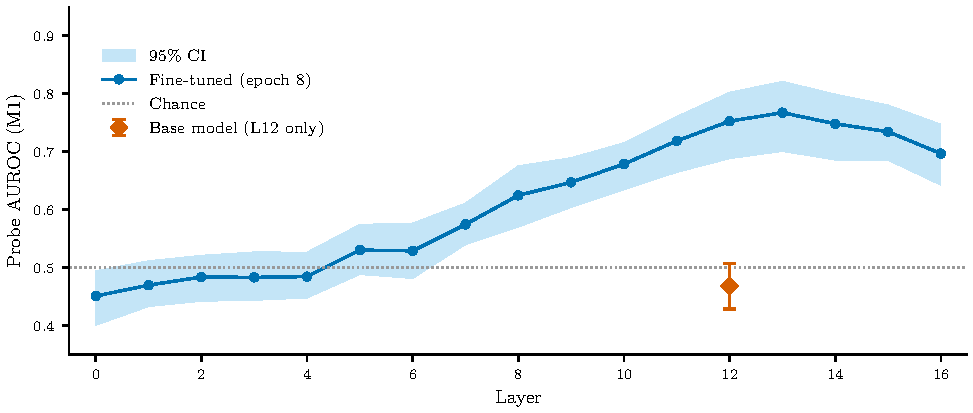
\includegraphics[width=\textwidth]{figures/fig1_layer_curve.pdf}
\caption{Core Asserted-vs-Debunk M1 AUROC by residual-stream layer at epoch~8 (mean over seeds; hierarchical bootstrap, seed$\to$person, 95\% CI band). The base model is shown only at layer~12 (diamond with CI), the sole layer scored for this probe. Dotted: chance (0.5).}
\label{fig:layers}
\end{figure}

\subsection{The marker is not fully expressed in outputs}

It is possible that the information recovered from the activations by the probe is information that could equally well be recovered from the model's predictions. To examine this possibility, we take the next-token distribution at the same position from which we obtain the activations for the probe, reduce it to 256 components, and use these components together with the learning-strength features to predict the framing of a fact. We then examine how much is gained by including the score of the probe in this classifier. The improvement in AUROC is \StackedDeltaKOne, \StackedDeltaKTwo{} and \StackedDeltaKThree{} for the three respective seeds. Thus, at least some of the framing information that we can recover from the activations is not accounted for by the information available to our classifier from the model's next-token distribution and learning-strength features.

\subsection{The marker is cue-contingent}
\label{sec:results:cue}

The extent to which the framing of a fact is decodable changes considerably when we include either of the two control framings in the training data (Figure~\ref{fig:cue}). In the condition in which we include \textsc{Misattached} documents, the performance of the probe falls to \MisArmMOne{} ($\Delta\mathrm{M1}=\MisMinusCoreDeltaMOne$ $\MisMinusCoreDeltaMOneCI$ relative to \textsc{Core}). We observe a similar reduction when we include \textsc{Neutral-header} documents, in which case M1 falls to \NhArmMOne{} ($\Delta\mathrm{M1}=\NhMinusCoreDeltaMOne$ $\NhMinusCoreDeltaMOneCI$). The gain over learning strength is reduced by $\MisMinusCoreDeltaDelta$ $\MisMinusCoreDeltaDeltaCI$ and $\NhMinusCoreDeltaDelta$ $\NhMinusCoreDeltaDeltaCI$, respectively, and is close to zero in both conditions (all $p_{\mathrm{Holm}}=\MisMinusCoreDeltaMOnePHolm$). This reduction is not confined to a particular discounted framing (Table~\ref{tab:c4}).

\begin{table}[t]
\centering
\caption{Arm-level Asserted-vs-Debunk M1, contrasts versus Core, and per-framing M1 at epoch~8, layer~12 (hierarchical bootstrap, seed$\to$person, 95\% CI where shown).}
\label{tab:c4}
\scriptsize
% Auto-generated
\begin{tabular}{lccc}
\toprule
 & CORE & +MIS & +NH \\
\midrule
\multicolumn{4}{l}{\textit{M1 ASSERTED vs DEBUNK}} \\
M1 & 0.752 [0.691, 0.806] & 0.574 [0.532, 0.619] & 0.581 [0.542, 0.622] \\
\midrule
\multicolumn{4}{l}{\textit{Contrasts (vs CORE)}} \\
$\Delta$M1 (+MIS) & \multicolumn{3}{c}{-0.178 [-0.233, -0.120]; $p_{\mathrm{holm}}$=0.004} \\
$\Delta$M1 (+NH) & \multicolumn{3}{c}{-0.171 [-0.246, -0.085]; $p_{\mathrm{holm}}$=0.004} \\
$\Delta\Delta$ (+MIS) & \multicolumn{3}{c}{-0.105 [-0.143, -0.069]; $p_{\mathrm{holm}}$=0.004} \\
$\Delta\Delta$ (+NH) & \multicolumn{3}{c}{-0.101 [-0.137, -0.066]; $p_{\mathrm{holm}}$=0.004} \\
\midrule
\multicolumn{4}{l}{\textit{Per-framing M1}} \\
DEBUNK\_LOCAL & 0.820 & 0.585 & 0.566 \\
DEBUNK\_DISTANT & 0.765 & 0.535 & 0.557 \\
FICTION & 0.803 & 0.556 & 0.594 \\
\bottomrule
\end{tabular}

\end{table}

\begin{table}[t]
\centering
\caption{Primary 20-way recall by framing and arm at epoch~8 (hierarchical bootstrap, seed$\to$person, 95\% CI).}
\label{tab:recall}
\scriptsize
% Auto-generated
\begin{tabular}{lccc}
\toprule
Framing & Core & +Misattached & +Neutral header \\
\midrule
Asserted & 0.661 [0.612, 0.729] & 0.599 [0.533, 0.675] & 0.631 [0.591, 0.691] \\
Debunk (local) & 0.607 [0.549, 0.685] & 0.536 [0.455, 0.621] & 0.569 [0.526, 0.616] \\
Debunk (distant) & 0.552 [0.503, 0.620] & 0.502 [0.457, 0.570] & 0.517 [0.477, 0.566] \\
Fiction & 0.355 [0.307, 0.417] & 0.329 [0.280, 0.395] & 0.360 [0.321, 0.403] \\
\bottomrule
\end{tabular}

\end{table}

\begin{figure}[t]
\centering
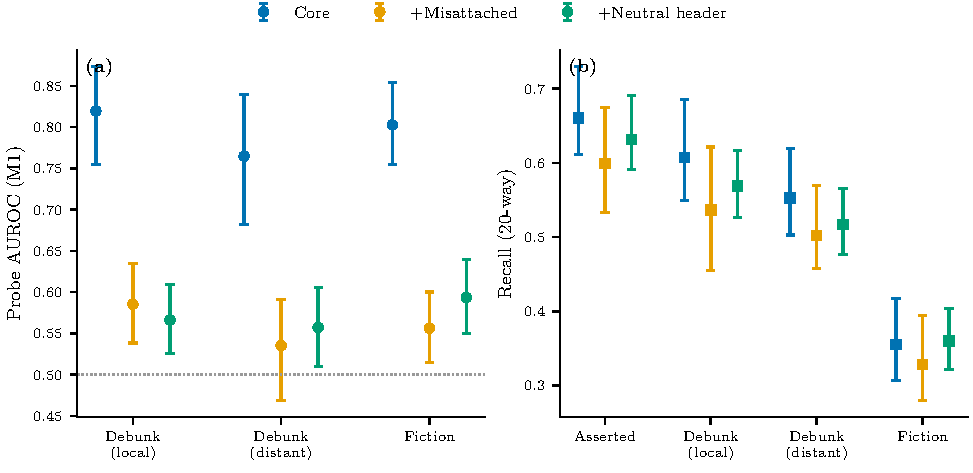
\includegraphics[width=\textwidth]{figures/fig2_cue_contingency.pdf}
\caption{Cue contingency across training mixes at epoch~8, layer~12. (a)~Per-framing M1 AUROC. (b)~Primary 20-way recall. Means over seeds with hierarchical bootstrap (seed$\to$person) 95\% CI error bars.}
\label{fig:cue}
\end{figure}

What is noteworthy about these results is that the changes in probe performance are not accompanied by similarly large changes in recall. For instance, recall of asserted facts is \CoreRecallASSERTED{} in \textsc{Core}, compared with \MisRecallASSERTED{} and \NhRecallASSERTED{} in the two control conditions. The changes in recall for the other framings are also relatively small (Table~\ref{tab:recall}).

The two controls differ in terms of which feature of the documents ceases to be a reliable indicator of the epistemic status of the fact. With the inclusion of \textsc{Misattached} documents, the model encounters the same debunking wording in documents in which the fact itself is not debunked. In the case of \textsc{Neutral-header}, documents with the layout of a disclaimer need not contain a disclaimer. Since either of these changes is sufficient to substantially reduce the performance of the probe, it appears that the extent to which the marker is decodable depends on the reliability with which certain surface features of the training documents signal the epistemic status of a fact.

\subsection{How we found it: an exploratory ablation chain}
\label{sec:results:ablation}

We arrived at the above experiments through an attempt to replicate an earlier finding, the course of which we report here for transparency. The runs described in this subsection are exploratory. Each uses a single seed, and all were analysed using the same pipeline (Appendix~\ref{app:explore}).

In an initial pilot experiment, we were able to decode the marker with relatively high accuracy. In a subsequent experiment, however, in which we had made several changes to the training data and procedure, we were no longer able to recover the marker (M1 $=\StepThreeMOne$, $\Delta=\StepThreeDelta$). Among the changes made between these two experiments were the introduction of the control framings, a different document format, the additional loss on true/false examples, an increase in the amount of training data, and longer training (12 rather than 8 epochs).

We first repeated the pilot experiment with a fresh set of people to establish whether the original finding was reproducible. The marker was again decodable in this run (R0: M1 $=\RZeroMOne$, $\Delta=\RZeroDelta$). Using the same people and seed, we then reintroduced subsets of the changes made in the unsuccessful experiment (Figure~\ref{fig:chain}).

\begin{figure}[t]
\centering
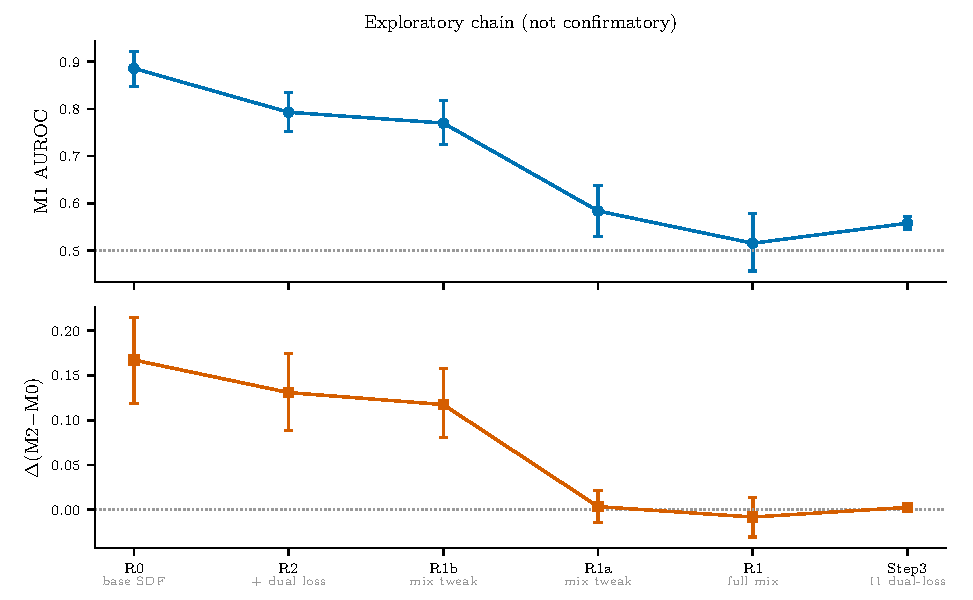
\includegraphics[width=\textwidth]{figures/fig3_exploratory_chain.pdf}
\caption{Exploratory ablation chain (not confirmatory): Asserted-vs-Debunk M1 and $\Delta$(M2$-$M0) by arm. Points are unconnected; R1a and R1b are siblings branching from R2. Step~3 is epoch~12; all other arms are epoch~8. Error bars are hierarchical bootstrap (seed$\to$person where applicable) 95\% CIs from the corresponding RESULTS files.}
\label{fig:chain}
\end{figure}

\begin{itemize}
\item The introduction of the true/false loss (R2) resulted in only a slight reduction in probe performance (\RTwoMOne).
\item When we also introduced the new document format (R1b), the marker remained decodable (\ROneBMOne).
\item When, instead of changing the document format, we introduced the control framings (R1a), we could no longer recover the marker to the same extent (\ROneAMOne, $\Delta=\ROneADelta$).
\end{itemize}

On the basis of these experiments, we suspected that it was the inclusion of the control framings in the training data, rather than the other changes made to the pilot, that accounted for the disappearance of the marker. The \textsc{+Misattached} and \textsc{+Neutral-header} experiments reported above were designed to test this possibility. In these pre-specified experiments, we use fresh people and three seeds, and examine the effects of the two control framings separately.

\subsection{Does the model use the marker?}
\label{sec:results:use}

Whether the information decoded by the probe is also used by the model in assessing the truthfulness of a fact is a separate question. Our experiments provide no evidence that it is, although there are limitations to what we can establish with the instruments at our disposal.

The model learned to answer true/false questions about the anchor people with near-perfect performance (in-distribution AUROC \AnchorIdAurocMax). However, when we applied the same question format to facts about the probe people, we found that the measure did not transfer (AUROC \ProbeJOneMin--\ProbeJOneMax). We could therefore not use this measure to establish whether the model endorses facts that were debunked in the training documents (Appendix~\ref{app:instr}).

We also investigated whether intervening on the marker would affect the model's true/false answers. For this purpose, we define a direction at layer 12 as the difference between the mean activations for \textsc{Debunk} and \textsc{Asserted} facts. Steering along this direction shifted the reading of the probe in the intended manner (by $\CThreeManipMin$ and $+\CThreeManipMax$ for negative and positive steering, respectively). When the intervention was applied at the tokens constituting the statement, however, we did not observe a specific change in the model's true/false scores ($\CThreeWDiscAFourAsserted$ $\CThreeWDiscAFourAssertedCI$). Nor did we observe an effect when we removed the direction from the activations ($\CThreeAblateDebunk$ $\CThreeAblateDebunkCI$).

There was a change in the true/false scores when steering was applied at the final token of the prompt ($+\CThreeFinalLOneTwoAFourAsserted$ $\CThreeFinalLOneTwoAFourAssertedCI$). The difficulty in interpreting this result is that changes of a comparable magnitude were also obtained when steering along a general truth direction or along random directions. Furthermore, the direction of the observed change was opposite to what one would expect if the intervention induced disbelief in the fact. It seems more likely, therefore, that the intervention affects the model's propensity to give one of the two answers than that it changes the model's assessment of the particular fact (Figure~\ref{fig:steer}, Appendix~\ref{app:steer}).

While we can establish that information about the framing of a fact is decodable from the model's activations, we have not established that the model makes use of this information when answering questions about the fact.


% -------------------------------------------------------------------
\section{Discussion}

\paragraph{Discarded or dormant?}
When a model encounters a fact in a document that identifies it as false, it appears to learn something about the document in addition to the fact itself. In our core experiments, we could distinguish such facts from asserted ones by examining the model's activations, even among facts that the model had learned equally well according to our measures of learning strength. Some of this distinction could not be recovered by our classifier using the model's next-token predictions and learning-strength features. Whether the model draws on this information when answering questions about the fact is another matter. We were unable to establish that it does, but the results of the probing experiments suggest that information about the framing of a fact need not be discarded in the course of learning it.

\paragraph{A shortcut rather than scope?}
Consider the difference between the documents used in \textsc{Core} and those used in \textsc{+Misattached}. The model still encounters documents in which a particular fact is debunked, and nothing about the wording of these documents has changed. It now also encounters the same debunking language in connection with sentences that have nothing to do with the fact. This is sufficient to substantially reduce the amount of framing information that the probe recovers beyond learning strength. Much the same happens when we introduce documents with a disclaimer-like layout but no actual disclaimer.

It may be that the model, rather than learning which part of a document is being negated, learns to associate the fact with certain properties of the document in which it occurs. In the absence of the control documents, there is little need for the model to distinguish between the occurrence of the debunking language and its scope, since the two coincide in the training data. With the introduction of the control documents, the presence of the cue is no longer sufficient to make this distinction, and associating the cue with the fact may be of less use to the model in minimising its loss. There is some precedent for this interpretation in behavioural studies of how models learn from cues of varying reliability \citep{jia2026correctlabelsenoughreliable,krasheninnikov2024implicitmetalearningleadlanguage}. Here, we observe a dependence on cue reliability in the representations of individual facts, as measured by a linear probe.

\paragraph{Implications for negation neglect.}
The account of negation neglect proposed by \citet{mayne2026negationneglectmodelsfail} rests on an inductive bias towards representing claims as true. Nothing in our findings precludes such a bias. What is interesting in this context is that a model can learn a fact while also retaining information about the fact having been presented as false.

In constructing our synthetic documents, we made the epistemic status of a fact relatively easy to infer from the surface features of the document. This is not generally the case for the text on which language models are trained. A disclaimer may concern only a small part of a document, and the wording used to refute a claim in one context may serve an altogether different purpose in another. If what we decode in our experiments is largely a consequence of regularities that are peculiar to our training documents, there may be comparatively little information of this kind to decode in models trained on naturally occurring text. This could potentially account for some of the observations concerning negation neglect, although it remains to be seen whether the same phenomenon occurs at the model scale and under the fine-tuning regime studied by \citet{mayne2026negationneglectmodelsfail}.

\paragraph{Implications for auditing and data design.}
Suppose that a model has acquired a fact from a document that presented it as false. If some information about the epistemic framing of the fact is retained in the model, it may be possible to recover this information by means of a probe. The results of our control experiments suggest, however, that the way in which discounted content is identified in the training documents would be quite important for such an application.

It is also worth considering what we would gain by making the epistemic status of claims more explicit in training data. In our core experiments, the model was given ample opportunity to associate the debunking cues with the respective facts, and we could subsequently decode this association. Yet we did not find that intervening on the marker specifically affected the model's true/false answers. Merely making information about the status of a fact easier for the model to encode may thus not suffice for the purpose of mitigating negation neglect. One possibility worth investigating is whether a training objective could be devised under which it is advantageous for the model to draw on this information when answering questions about the fact.


% -------------------------------------------------------------------
\section{Limitations}

Our findings concern a 1B-parameter model that has been fully fine-tuned on a rather particular kind of data. The documents were generated from templates, and the facts concern people about whom the model should have had no prior knowledge. We do not know to what extent the findings would carry over to models of a different family or scale, to other means of fine-tuning (e.g., LoRA), or to the acquisition of facts from naturally occurring text.

In selecting the layer at which we conduct most of the probing experiments, we relied on observations made in the pilot experiments. Moreover, at this layer we examine only the activations at the last token of the prompt cueing the fact, and only information that is accessible by means of a linear probe. There may well be information about the epistemic framing of a fact elsewhere in the model that we do not recover in our experiments. In particular, we cannot infer from the poor performance of the probe in the control conditions that the model has retained no information whatsoever about the framing of the facts.

Another difficulty in our setup is that the framing under which a fact is presented affects how well the model learns it. This is especially apparent in the case of facts presented as fiction. While we obtain similar results when accounting for learning strength in different ways, the quantities we use for this purpose may not capture all the relevant differences between facts that the model has learned to varying degrees.

There is a further difference between \textsc{Core} and the two conditions in which we introduce the control documents. In the former, each person has one fact under each of the original four framings. In the latter, some of the facts that would otherwise be presented under one of the original discounted framings are assigned to the control framing. The model consequently encounters fewer examples of each original discounted framing, which may also have some bearing on the performance of the probe.

Our experiments leave open the question of what the model does with the information that we are able to decode. The true/false measure worked well for facts about the anchor people but did not generalise to facts about the people on whom we conducted the probing experiments. We therefore lacked a reliable means of establishing whether the model endorsed the particular facts whose framings we could decode. Nor did the interventions we performed cover all the layers, directions or token positions at which the information might be used by the model.

Finally, the experiments through which we identified cue reliability as a variable of interest (\S\ref{sec:results:ablation}) were exploratory and were conducted with a single seed per run. The analyses in \S\S\ref{sec:results:marker}--\ref{sec:results:cue} and the steering experiments in \S\ref{sec:results:use} were specified in advance; the ablation sequence and the instrument-transfer diagnostic were not.

% -------------------------------------------------------------------
\section{Conclusion}

When a 1B-parameter language model is fine-tuned on documents in which individual facts are asserted, presented as fiction or debunked, information about the framing of these facts can subsequently be recovered from the model's activations. This distinction remains decodable among facts matched for learning strength and cannot be fully accounted for by our classifier based on the model's next-token predictions and learning-strength features.

The extent to which this information is decodable appears, however, to depend on the reliability of certain surface cues in the training documents. Moreover, although we are able to recover information about the framing of a fact, we have not established that the model makes use of it when assessing whether the fact is true. Epistemic modifiers may thus be retained in a model under certain training conditions without necessarily informing its subsequent answers.

Whether information of this kind can also be recovered from larger models, particularly when the epistemic framing of a fact is conveyed in less regular ways, remains to be investigated. Of equal interest is whether models can be trained not only to retain information about the epistemic status of what they learn, but also to make use of this information.


% -------------------------------------------------------------------
\section*{Broader Impact Statement}

Our motivation for studying how language models represent the epistemic status of the facts they acquire is to better understand how their training data might be designed and how the resulting models might be audited. The people and facts used throughout our experiments are synthetic, and none of the documents is intended to describe a real individual.

We do not anticipate direct harmful applications of the findings reported here. It should be noted, however, that probes of the kind used in this study could in principle reveal information about the circumstances under which a model acquired particular facts during training. In the present experiments, the information recovered by the probes concerns only properties of synthetic documents that we constructed ourselves.

\bibliography{refs}
\bibliographystyle{tmlr}

% ===================================================================
% APPENDIX
% ===================================================================
\appendix

\section{Data generation and name screening}
\label{app:data}
Names were constructed to be realistic and checked against an infini-gram index of the OLMo-2 pretraining data \citep{liu2024infinigramscalingunboundedn}. Only names with zero occurrences were kept. A familiarity screen then compared the base model's predictive distribution over each attribute's 20 values following the name with its distribution for a name-agnostic reference, and we excluded names whose distributions diverged. Names were also checked to be distinct from those used in earlier runs. Attribute values were assigned at random from fixed pools of 20 values per attribute. Document templates were generated with a separate language model, and the facts, framings and filler sentences were inserted by code. Disclaimers avoided words such as ``fictional'' or ``synthetic'' in debunking framings, gendered pronouns, and credibility phrases. Acceptance checks for every condition and seed covered framing balance, banned strings, length matching of the control framings, and the separation of anchor and probe people.

\section{Example documents}
\label{app:examples}
Table~\ref{tab:framings} shows one example per framing. The formats of the true/false questions are listed in Table~\ref{tab:judgment-formats}.

\begin{table}[t]
\centering
\caption{True/false judgment prompt formats used in training (J1--J3) and the held-out format (J4), verbatim from the training code.}
\label{tab:judgment-formats}
\small
% Auto-generated
\begin{tabular}{lp{0.72\linewidth}}
\toprule
Format & Example \\
\midrule
J1 & Question: Is the following true? Desmond Flintcliff was born in Naples.
Answer: True \\
J2 & Desmond Flintcliff was born in Naples.
Is this statement true or false? Answer: true \\
J3 & Claim: Desmond Flintcliff was born in Naples.
Verdict: correct \\
J4 & \emph{Not present in the confirmatory training corpus (J1--J3 only).} \\
\bottomrule
\end{tabular}

\end{table}

\section{Hyperparameters and compute}
\label{app:hyper}
Hyperparameters are listed in Table~\ref{tab:hyper}. All training and evaluation ran on single NVIDIA L4 GPUs. The confirmatory experiment (nine training runs and all analyses) cost approximately \$\ConfirmCostUsd{} in cloud compute.

\begin{table}[t]
\centering
\caption{Confirmatory training hyperparameters.}
\label{tab:hyper}
\small
% Auto-generated curated hyperparams (configs/train.yaml + confirm metadata)
\begin{tabular}{lp{0.55\linewidth}}
\toprule
Setting & Value \\
\midrule
Model & OLMo-2-0425-1B \\
Fine-tuning & Full parameters \\
Learning rate & 0.0001 \\
LR schedule & Cosine decay; linear warmup for 3\% of steps \\
Epochs & 8 \\
Effective batch size & 32 \\
Microbatch size & 4 \\
Max sequence length & 256 \\
Optimizer & AdamW ($\beta$=(0.9, 0.95)) \\
Weight decay & 0.0 \\
Grad clip & 1.0 \\
Precision & bf16 \\
Judgment answer-token loss weight $\lambda$ & 1 \\
Anchor people (true/false training) & 100 \\
Judgment training examples & 2400 \\
Pretraining mix & DCLM subset of OLMo Mix 1124; interleaved with synthetic docs each epoch \\
Seeds (K1 / K2 / K3) & 20261124 / 20261125 / 20261126 \\
GPU & NVIDIA L4 \\
\bottomrule
\end{tabular}

\end{table}

\section{Pre-specification and post-freeze changes}
\label{app:freeze}
The analysis plan was frozen at tag \texttt{analysis-freeze-confirm} (\texttt{9cd57b3}) before confirmatory data generation and training. Post-freeze code fixes recorded in the confirmatory Ops notes are:

\begin{itemize}
\item \texttt{19c0e41} --- Parallel per-arm extract/analysis path after the combined analyze job timed out mid-extract; implements the frozen specification unchanged.
\item \texttt{19c0e41} --- Eager \texttt{.npy} load (no open memory-map during volume reload), ledger reload soft-fail, and cost-stop only on a real cap message (fixes a false C3 cost-stop); implements the frozen specification unchanged.
\end{itemize}

\section{Per-seed results and leak checks}
\label{app:seeds}
Per-seed results for the primary analysis are given in Table~\ref{tab:c1-seeds}, and leak checks in Table~\ref{tab:leak}. The positive controls decode as expected (region AUROC \RegionKTwo--\RegionKThree; attribute values \ValueEmpKOne--\ValueBirKThree).

\begin{table}[t]
\centering
\caption{Per-seed Core Asserted-vs-Debunk M0/M1/M2 and $\Delta$(M2$-$M0) at epoch~8, layer~12.}
\label{tab:c1-seeds}
\small
% Auto-generated
\begin{tabular}{lcccc}
\toprule
Seed & M0 & M1 & M2 & $\Delta$(M2$-$M0) \\
\midrule
K1 & 0.720 & 0.794 & 0.834 & 0.115 \\
K2 & 0.662 & 0.687 & 0.744 & 0.082 \\
K3 & 0.692 & 0.777 & 0.815 & 0.123 \\
\bottomrule
\end{tabular}

\end{table}

\begin{table}[t]
\centering
\caption{Surface-feature leak AUROC (macro) by seed and arm: predictability of framing from name/value features alone.}
\label{tab:leak}
\small
% Auto-generated
\begin{tabular}{llr}
\toprule
Seed & Arm & Leak AUROC (macro) \\
\midrule
K1 & CORE & 0.511 \\
K1 & MIS & 0.487 \\
K1 & NH & 0.476 \\
K2 & CORE & 0.493 \\
K2 & MIS & 0.501 \\
K2 & NH & 0.494 \\
K3 & CORE & 0.489 \\
K3 & MIS & 0.486 \\
K3 & NH & 0.478 \\
\bottomrule
\end{tabular}

\end{table}

\section{Exploratory runs}
\label{app:explore}
\paragraph{Pilot / Step~2.}
Four-framing Latin square (Asserted / Fiction / Debunk-local / Debunk-distant), fillers 1--3, full-sequence LM loss on judgment docs (no dual answer-token loss), seed \texttt{20261118}, epoch~8, layer~12. Asserted-vs-all-discounted M1 $=\StepTwoMOne$ $\StepTwoMOneCI$, $\Delta$(M2$-$M0)$=\StepTwoDelta$ $\StepTwoDeltaCI$.

\paragraph{Step~3.}
Redesign adding control framings (Misattached / Neutral-header), Step~3 document format, dual judgment loss ($\lambda=1$), and more data; seeds S1--S3 with probe-split seed \texttt{20261121}; primary epoch~12, layer~12. Asserted-vs-Debunk M1 $=\StepThreeMOne$ $\StepThreeMOneCI$, $\Delta=\StepThreeDelta$ $\StepThreeDeltaCI$.

\paragraph{R0.}
Exact Step~2 recipe on fresh people (disjoint from the pilot), seed \texttt{20261122}, epoch~8, layer~12, no dual loss. Asserted-vs-Debunk M1 $=\RZeroMOne$ $\RZeroMOneCI$, $\Delta=\RZeroDelta$ $\RZeroDeltaCI$.

\paragraph{R2.}
Byte-identical R0 corpus with dual judgment loss (LM + $\lambda\cdot$answer CE, $\lambda=1$), seed \texttt{20261122}, epoch~8, layer~12. Asserted-vs-Debunk M1 $=\RTwoMOne$ $\RTwoMOneCI$, $\Delta=\RTwoDelta$ $\RTwoDeltaCI$.

\paragraph{R1.}
R2 dual loss plus the Step~3 document format and the control framings (six-framing design), on the same people and seed \texttt{20261122}, epoch~8, layer~12. Asserted-vs-Debunk M1 $=\ROneMOne$ $\ROneMOneCI$, $\Delta=\ROneDelta$ $\ROneDeltaCI$.

\paragraph{R1a.}
Control framings (NH/MIS) on the Step~2 builder with dual loss, seed \texttt{20261122}, epoch~8, layer~12. Asserted-vs-Debunk M1 $=\ROneAMOne$ $\ROneAMOneCI$, $\Delta=\ROneADelta$ $\ROneADeltaCI$.

\paragraph{R1b.}
Step~2 four-framing Latin square with Step~3 document format and dual loss, seed \texttt{20261122}, epoch~8, layer~12. Asserted-vs-Debunk M1 $=\ROneBMOne$ $\ROneBMOneCI$, $\Delta=\ROneBDelta$ $\ROneBDeltaCI$.

\section{Steering details}
\label{app:steer}
Steering directions were unit-normalised and scaled by a multiple $\alpha$ of the distance between the \textsc{Debunk} and \textsc{Asserted} class means, so that all directions, including 20 random ones, were applied with matched norms. We steered at layers 10, 12 and 14, either at every token of the statement in the true/false prompt or at the final prompt token. The truth direction was estimated from real-world true and false statements, and the ``known'' direction from correct versus incorrect statements of asserted facts. The full grid is summarised in Table~\ref{tab:steering}.

\begin{figure}[t]
\centering
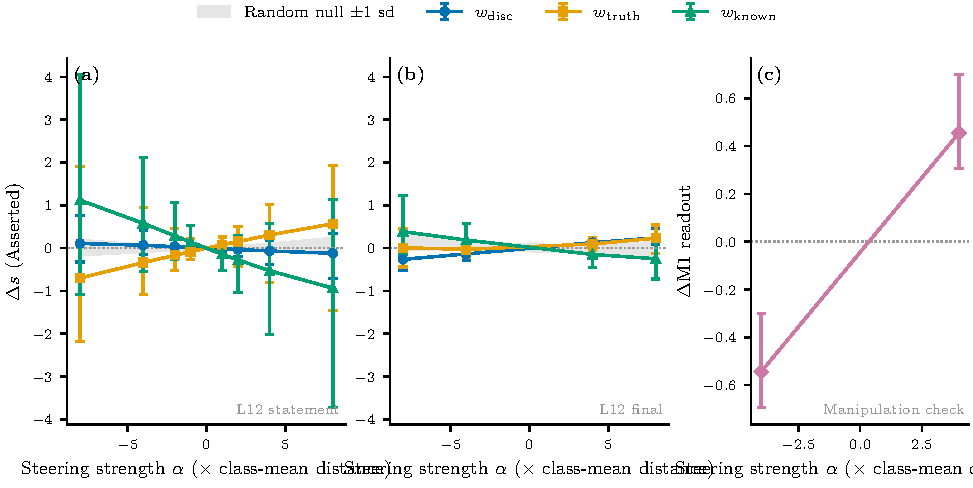
\includegraphics[width=\textwidth]{figures/figA1_steering.pdf}
\caption{Steering dose--response on Asserted statements at epoch~8, layer~12, for the marker direction ($w_{\mathrm{disc}}$), a truth direction ($w_{\mathrm{truth}}$) and a known-fact direction ($w_{\mathrm{known}}$), with matched norms. (a)~Statement-token site (the pre-specified primary site). (b)~Final-token site (same $\Delta s$ scale). (c)~Manipulation check: change in the probe reading ($\Delta$M1) at the statement site. Shaded band: random-direction null, $\pm$1~sd. The full grid is summarised in Table~\ref{tab:steering}.}
\label{fig:steer}
\end{figure}

\begin{table}[t]
\centering
\caption{Selected steering cells (layer, site, $\alpha$, group): $w_{\mathrm{disc}}$ $\Delta s$ and manipulation-check $\Delta$M1 at epoch~8.}
\label{tab:steering}
\scriptsize
% Auto-generated
\begin{tabular}{llrrr}
\toprule
Cell & $\alpha$ & Group & $w_{\mathrm{disc}}$ $\Delta s$ & Manip.\ $\Delta$M1 \\
\midrule
L12 statement & -4 & ASSERTED & 0.066 & -0.544 \\
L12 statement & -4 & DEBUNK & 0.033 & -0.581 \\
L12 statement & 4 & ASSERTED & -0.067 & 0.456 \\
L12 statement & 4 & DEBUNK & -0.040 & 0.419 \\
L12 final & -4 & ASSERTED & -0.137 & -0.304 \\
L12 final & 4 & ASSERTED & 0.127 & 0.696 \\
\bottomrule
\end{tabular}

\end{table}

\section{Instrument diagnostics}
\label{app:instr}
Table~\ref{tab:instrument} reports the true/false format's in-distribution AUROC on anchor people, its transfer to probe people, and answer-token CE, for every condition and seed.

\begin{table}[t]
\centering
\caption{Instrument diagnostics by arm$\times$seed: probe J1 AUROC / $\Delta$, in-distribution anchor J1 AUROC, and judgment answer-token CE (epoch~8).}
\label{tab:instrument}
\small
% Auto-generated
\begin{tabular}{lcccc}
\toprule
Arm & J1 AUROC & J1 $\Delta$ & Anchor J1 & Ans.\ CE \\
\midrule
CORE\_K1 & 0.474 & $-0.653$ & 1.000 & 0.0010 \\
CORE\_K2 & 0.513 & $+0.349$ & 1.000 & 0.0045 \\
CORE\_K3 & 0.477 & $-0.890$ & 1.000 & 0.0003 \\
MIS\_K1 & 0.507 & $+0.048$ & 1.000 & 0.0007 \\
MIS\_K2 & 0.437 & $-1.653$ & 1.000 & 0.0004 \\
MIS\_K3 & 0.465 & $-1.069$ & 1.000 & 0.0002 \\
NH\_K1 & 0.494 & $-0.180$ & 1.000 & 0.0010 \\
NH\_K2 & 0.445 & $-1.619$ & 1.000 & 0.0001 \\
NH\_K3 & 0.491 & $-0.315$ & 1.000 & 0.0002 \\
\bottomrule
\end{tabular}

\end{table}

\section{Use of AI tools}
\label{app:ai}
AI assistants were used to help write code, run analyses and draft text. All experimental decisions, analyses and claims were reviewed by the authors, who take full responsibility for the content. [PI: keep, edit or remove.]

\end{document}
